% Options for packages loaded elsewhere
\PassOptionsToPackage{unicode}{hyperref}
\PassOptionsToPackage{hyphens}{url}
%
\documentclass[
]{book}
\usepackage{amsmath,amssymb}
\usepackage{lmodern}
\usepackage{iftex}
\ifPDFTeX
  \usepackage[T1]{fontenc}
  \usepackage[utf8]{inputenc}
  \usepackage{textcomp} % provide euro and other symbols
\else % if luatex or xetex
  \usepackage{unicode-math}
  \defaultfontfeatures{Scale=MatchLowercase}
  \defaultfontfeatures[\rmfamily]{Ligatures=TeX,Scale=1}
\fi
% Use upquote if available, for straight quotes in verbatim environments
\IfFileExists{upquote.sty}{\usepackage{upquote}}{}
\IfFileExists{microtype.sty}{% use microtype if available
  \usepackage[]{microtype}
  \UseMicrotypeSet[protrusion]{basicmath} % disable protrusion for tt fonts
}{}
\makeatletter
\@ifundefined{KOMAClassName}{% if non-KOMA class
  \IfFileExists{parskip.sty}{%
    \usepackage{parskip}
  }{% else
    \setlength{\parindent}{0pt}
    \setlength{\parskip}{6pt plus 2pt minus 1pt}}
}{% if KOMA class
  \KOMAoptions{parskip=half}}
\makeatother
\usepackage{xcolor}
\usepackage{color}
\usepackage{fancyvrb}
\newcommand{\VerbBar}{|}
\newcommand{\VERB}{\Verb[commandchars=\\\{\}]}
\DefineVerbatimEnvironment{Highlighting}{Verbatim}{commandchars=\\\{\}}
% Add ',fontsize=\small' for more characters per line
\usepackage{framed}
\definecolor{shadecolor}{RGB}{248,248,248}
\newenvironment{Shaded}{\begin{snugshade}}{\end{snugshade}}
\newcommand{\AlertTok}[1]{\textcolor[rgb]{0.94,0.16,0.16}{#1}}
\newcommand{\AnnotationTok}[1]{\textcolor[rgb]{0.56,0.35,0.01}{\textbf{\textit{#1}}}}
\newcommand{\AttributeTok}[1]{\textcolor[rgb]{0.77,0.63,0.00}{#1}}
\newcommand{\BaseNTok}[1]{\textcolor[rgb]{0.00,0.00,0.81}{#1}}
\newcommand{\BuiltInTok}[1]{#1}
\newcommand{\CharTok}[1]{\textcolor[rgb]{0.31,0.60,0.02}{#1}}
\newcommand{\CommentTok}[1]{\textcolor[rgb]{0.56,0.35,0.01}{\textit{#1}}}
\newcommand{\CommentVarTok}[1]{\textcolor[rgb]{0.56,0.35,0.01}{\textbf{\textit{#1}}}}
\newcommand{\ConstantTok}[1]{\textcolor[rgb]{0.00,0.00,0.00}{#1}}
\newcommand{\ControlFlowTok}[1]{\textcolor[rgb]{0.13,0.29,0.53}{\textbf{#1}}}
\newcommand{\DataTypeTok}[1]{\textcolor[rgb]{0.13,0.29,0.53}{#1}}
\newcommand{\DecValTok}[1]{\textcolor[rgb]{0.00,0.00,0.81}{#1}}
\newcommand{\DocumentationTok}[1]{\textcolor[rgb]{0.56,0.35,0.01}{\textbf{\textit{#1}}}}
\newcommand{\ErrorTok}[1]{\textcolor[rgb]{0.64,0.00,0.00}{\textbf{#1}}}
\newcommand{\ExtensionTok}[1]{#1}
\newcommand{\FloatTok}[1]{\textcolor[rgb]{0.00,0.00,0.81}{#1}}
\newcommand{\FunctionTok}[1]{\textcolor[rgb]{0.00,0.00,0.00}{#1}}
\newcommand{\ImportTok}[1]{#1}
\newcommand{\InformationTok}[1]{\textcolor[rgb]{0.56,0.35,0.01}{\textbf{\textit{#1}}}}
\newcommand{\KeywordTok}[1]{\textcolor[rgb]{0.13,0.29,0.53}{\textbf{#1}}}
\newcommand{\NormalTok}[1]{#1}
\newcommand{\OperatorTok}[1]{\textcolor[rgb]{0.81,0.36,0.00}{\textbf{#1}}}
\newcommand{\OtherTok}[1]{\textcolor[rgb]{0.56,0.35,0.01}{#1}}
\newcommand{\PreprocessorTok}[1]{\textcolor[rgb]{0.56,0.35,0.01}{\textit{#1}}}
\newcommand{\RegionMarkerTok}[1]{#1}
\newcommand{\SpecialCharTok}[1]{\textcolor[rgb]{0.00,0.00,0.00}{#1}}
\newcommand{\SpecialStringTok}[1]{\textcolor[rgb]{0.31,0.60,0.02}{#1}}
\newcommand{\StringTok}[1]{\textcolor[rgb]{0.31,0.60,0.02}{#1}}
\newcommand{\VariableTok}[1]{\textcolor[rgb]{0.00,0.00,0.00}{#1}}
\newcommand{\VerbatimStringTok}[1]{\textcolor[rgb]{0.31,0.60,0.02}{#1}}
\newcommand{\WarningTok}[1]{\textcolor[rgb]{0.56,0.35,0.01}{\textbf{\textit{#1}}}}
\usepackage{longtable,booktabs,array}
\usepackage{calc} % for calculating minipage widths
% Correct order of tables after \paragraph or \subparagraph
\usepackage{etoolbox}
\makeatletter
\patchcmd\longtable{\par}{\if@noskipsec\mbox{}\fi\par}{}{}
\makeatother
% Allow footnotes in longtable head/foot
\IfFileExists{footnotehyper.sty}{\usepackage{footnotehyper}}{\usepackage{footnote}}
\makesavenoteenv{longtable}
\usepackage{graphicx}
\makeatletter
\def\maxwidth{\ifdim\Gin@nat@width>\linewidth\linewidth\else\Gin@nat@width\fi}
\def\maxheight{\ifdim\Gin@nat@height>\textheight\textheight\else\Gin@nat@height\fi}
\makeatother
% Scale images if necessary, so that they will not overflow the page
% margins by default, and it is still possible to overwrite the defaults
% using explicit options in \includegraphics[width, height, ...]{}
\setkeys{Gin}{width=\maxwidth,height=\maxheight,keepaspectratio}
% Set default figure placement to htbp
\makeatletter
\def\fps@figure{htbp}
\makeatother
\setlength{\emergencystretch}{3em} % prevent overfull lines
\providecommand{\tightlist}{%
  \setlength{\itemsep}{0pt}\setlength{\parskip}{0pt}}
\setcounter{secnumdepth}{5}
\usepackage{booktabs}
\usepackage{amsthm}
\makeatletter
\def\thm@space@setup{%
  \thm@preskip=8pt plus 2pt minus 4pt
  \thm@postskip=\thm@preskip
}
\makeatother
\ifLuaTeX
  \usepackage{selnolig}  % disable illegal ligatures
\fi
\usepackage[]{natbib}
\bibliographystyle{apalike}
\IfFileExists{bookmark.sty}{\usepackage{bookmark}}{\usepackage{hyperref}}
\IfFileExists{xurl.sty}{\usepackage{xurl}}{} % add URL line breaks if available
\urlstyle{same} % disable monospaced font for URLs
\hypersetup{
  pdftitle={EcoSHEDS Northeast Brook Trout Occupancy Model},
  pdfauthor={Jeffrey D. Walker, Benjamin Letcher},
  hidelinks,
  pdfcreator={LaTeX via pandoc}}

\title{EcoSHEDS Northeast Brook Trout Occupancy Model}
\author{\href{https://walkerenvres.com}{Jeffrey D. Walker}, \href{https://www.usgs.gov/staff-profiles/benjamin-h-letcher}{Benjamin Letcher}}
\date{v2.0.0 (July 8, 2022)}

\begin{document}
\maketitle

{
\setcounter{tocdepth}{1}
\tableofcontents
}
\begin{verbatim}
## -- Attaching packages --------------------------------------- tidyverse 1.3.1 --
\end{verbatim}

\begin{verbatim}
## v ggplot2 3.3.6     v purrr   0.3.4
## v tibble  3.1.7     v dplyr   1.0.9
## v tidyr   1.2.0     v stringr 1.4.0
## v readr   2.1.2     v forcats 0.5.1
\end{verbatim}

\begin{verbatim}
## -- Conflicts ------------------------------------------ tidyverse_conflicts() --
## x dplyr::filter() masks stats::filter()
## x dplyr::lag()    masks stats::lag()
\end{verbatim}

\begin{verbatim}
## Linking to GEOS 3.9.1, GDAL 3.2.3, PROJ 7.2.1; sf_use_s2() is TRUE
\end{verbatim}

\begin{verbatim}
## Loading required package: lattice
\end{verbatim}

\begin{verbatim}
## 
## Attaching package: 'caret'
\end{verbatim}

\begin{verbatim}
## The following object is masked from 'package:purrr':
## 
##     lift
\end{verbatim}

\begin{verbatim}
## 
## Attaching package: 'janitor'
\end{verbatim}

\begin{verbatim}
## The following objects are masked from 'package:stats':
## 
##     chisq.test, fisher.test
\end{verbatim}

\hypertarget{intro}{%
\chapter{Introduction}\label{intro}}

The northeast brook trout occupancy model predicts the occupancy probability of eastern brook trout based on estimated stream temperatures across a high resolution catchment delineation for the northeast U.S. (Maine to Virginia). This model is developed and maintained as part of the \href{https://www.usgs.gov/apps/ecosheds/}{EcoSHEDS} project.

\hypertarget{model-summary}{%
\section{Model Summary}\label{model-summary}}

The occupancy model is a logistic linear mixed effects model for predicting occupancy probability based on estimated stream temperature. The primary model input is the estimated mean July stream temperature generated by the \href{https://ecosheds.org/models/stream-temperature/latest/}{EcoSHEDS Northeast Stream Temperature Model} and averaged over all years from 1980 to present. The model also includes a varying intercept (random effect) based on the HUC8\footnote{8-digit Hydrologic Unit Code (HUC)} basin containing each catchment to account for regional variations in occupancy not explained by stream temperature. Like the EcoSHEDS stream temperature model, the occupancy model domain is based on the \href{https://conte-ecology.github.io/shedsGisData/\#the-national-hydrography-dataset-high-resolution-delineation-version-2-nhdhrdv2}{EcoSHEDS Northeast Catchment Delineation}.

The occupancy model was calibrated using presence/absence data compiled from multiple state agencies across the region.

\begin{figure}
\centering
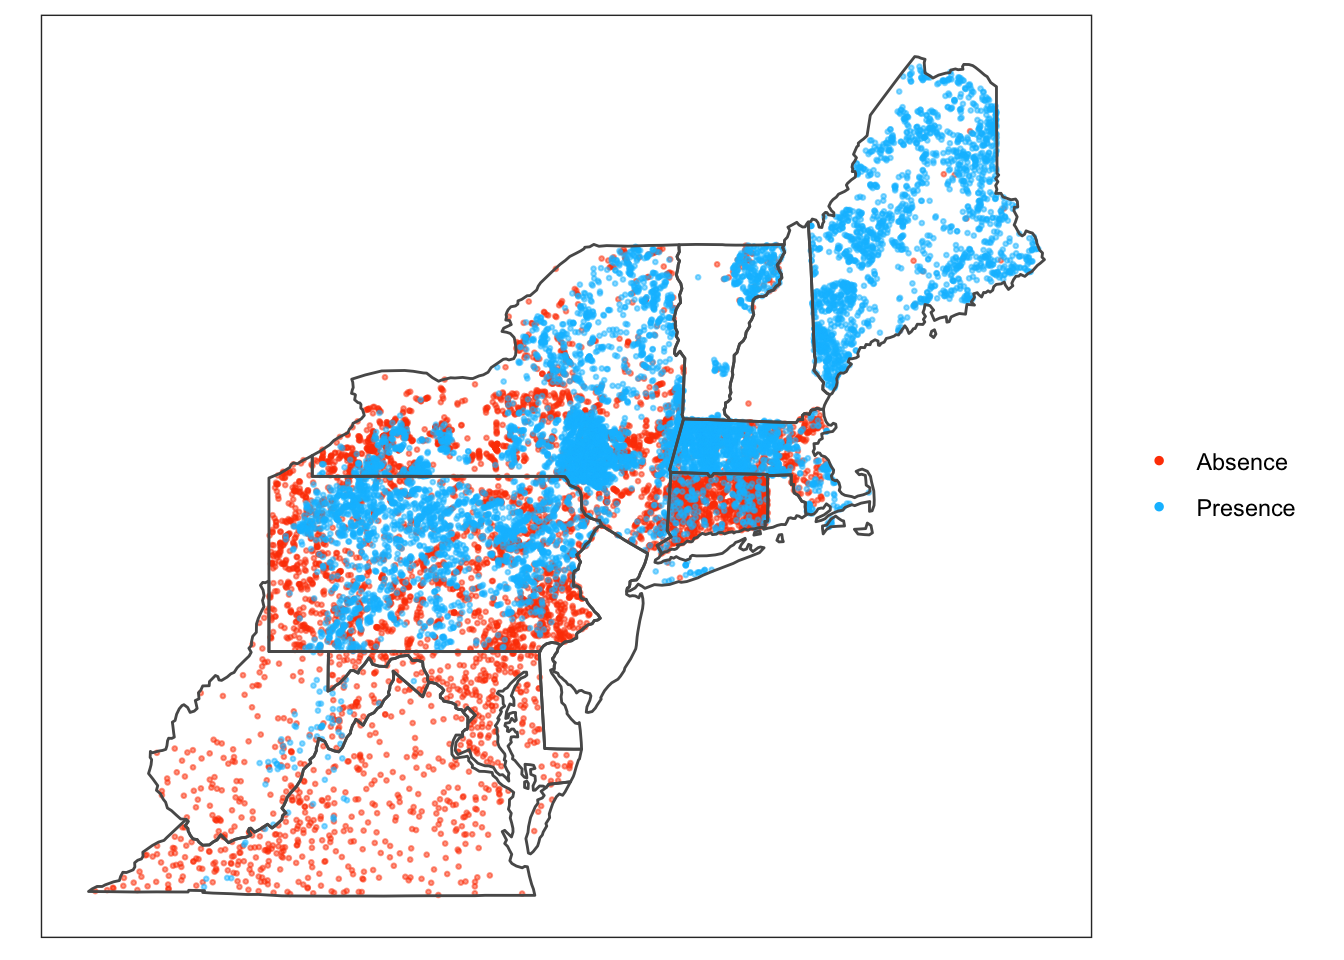
\includegraphics{sheds-bto-model_files/figure-latex/intro-obs-map-1.pdf}
\caption{\label{fig:intro-obs-map}Map of Presence/Absence by Catchment}
\end{figure}

The model was validating by splitting the observed presence/absence data into independent training and testing subsets, calibrating the model to the training data, and then comparing the model performance between the two subsets. The validation confirmed that the model structure is not susceptible to over-fitting. Following validation, the model was re-calibrated using all available observation data in order to maximize the amount of information used to generate the final predictions. The following table summarizes the model performance for each dataset.

\begin{tabular}{l|r|r|r}
\hline
Metric & Calibration & Validation & Full (Prediction)\\
\hline
Accuracy & 0.832 & 0.809 & 0.832\\
\hline
Sensitivity & 0.897 & 0.844 & 0.894\\
\hline
Specificity & 0.712 & 0.748 & 0.717\\
\hline
Pos Pred Value & 0.852 & 0.857 & 0.853\\
\hline
Neg Pred Value & 0.790 & 0.727 & 0.786\\
\hline
Precision & 0.852 & 0.857 & 0.853\\
\hline
Recall & 0.897 & 0.844 & 0.894\\
\hline
F1 & 0.874 & 0.850 & 0.873\\
\hline
Prevalence & 0.649 & 0.642 & 0.648\\
\hline
Detection Rate & 0.582 & 0.542 & 0.579\\
\hline
Detection Prevalence & 0.684 & 0.632 & 0.679\\
\hline
Balanced Accuracy & 0.805 & 0.796 & 0.806\\
\hline
\end{tabular}

Predicted occupancy probabilities were generated for each catchment under both historical conditions as well as for a series of simple climate change scenarios (e.g., +2, +4, +6 degC air temperature). Additional metrics were also computed to evaluate the vulnerability of brook trout occupancy within each catchment to climate change (e.g., the maximum air temperature increase that would result in 30, 50, or 70\% occupancy). Model predictions were only generated for catchments with cumulative drainage areas less than 200 km\textsuperscript{2} (i.e., lower order streams) due to the complexity of predicting stream temperatures in larger rivers.

\begin{figure}
\centering
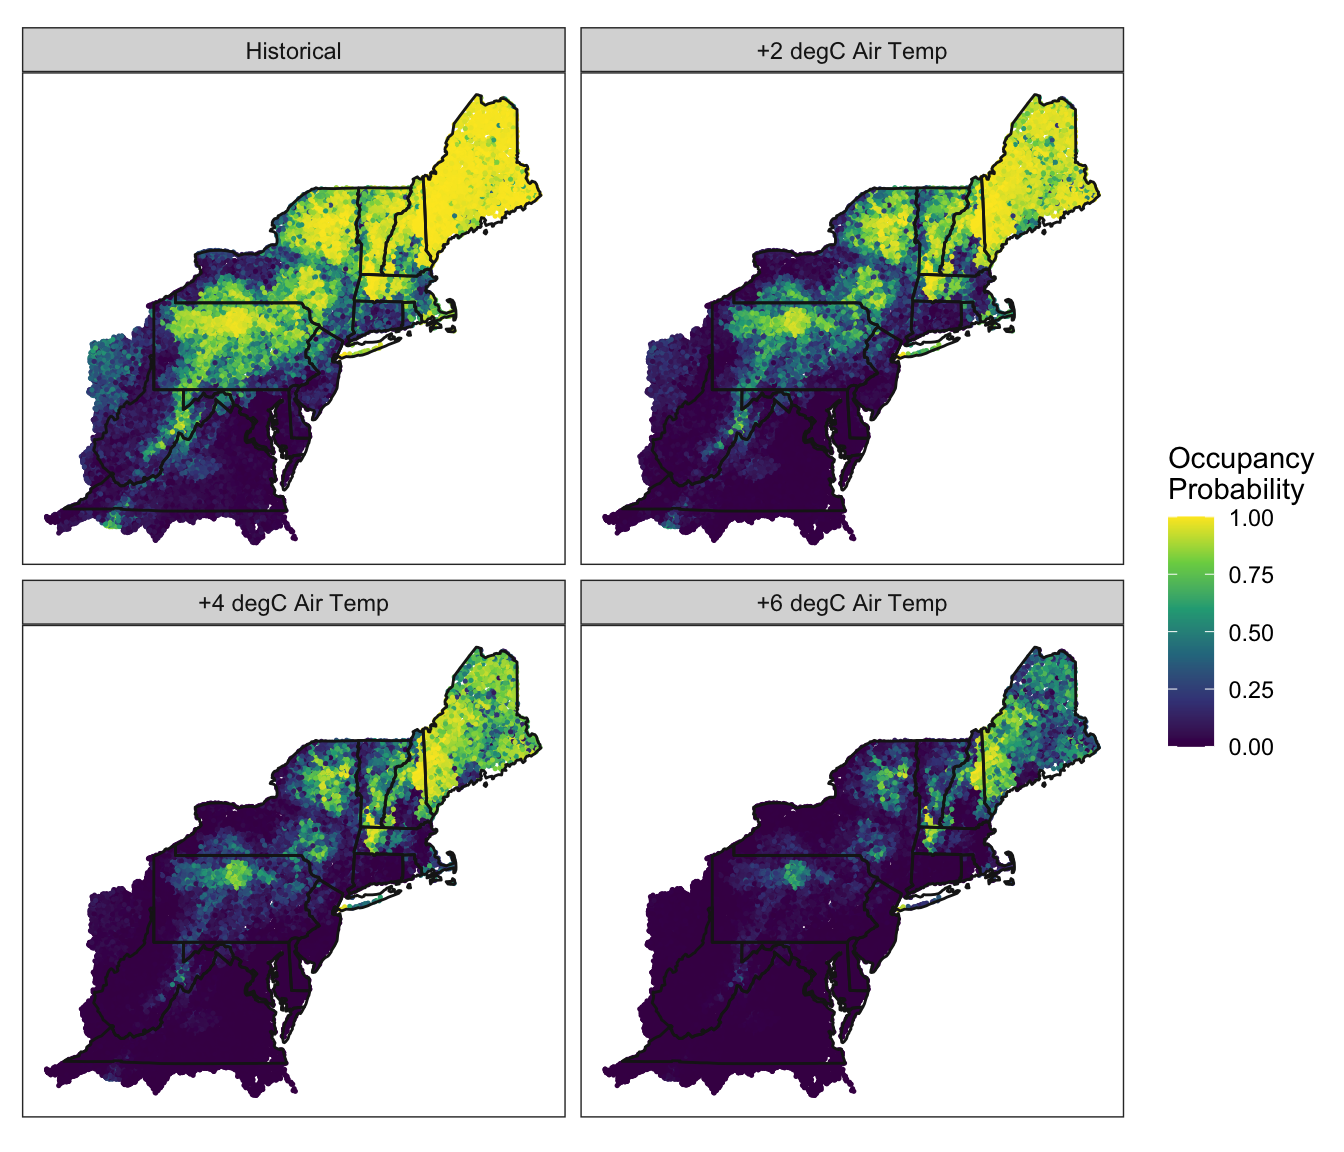
\includegraphics{sheds-bto-model_files/figure-latex/intro-map-prob-1.pdf}
\caption{\label{fig:intro-map-prob}Predicted Occupancy Probabilities under Historical and Future Climate Change Scenarios}
\end{figure}

\begin{figure}
\centering
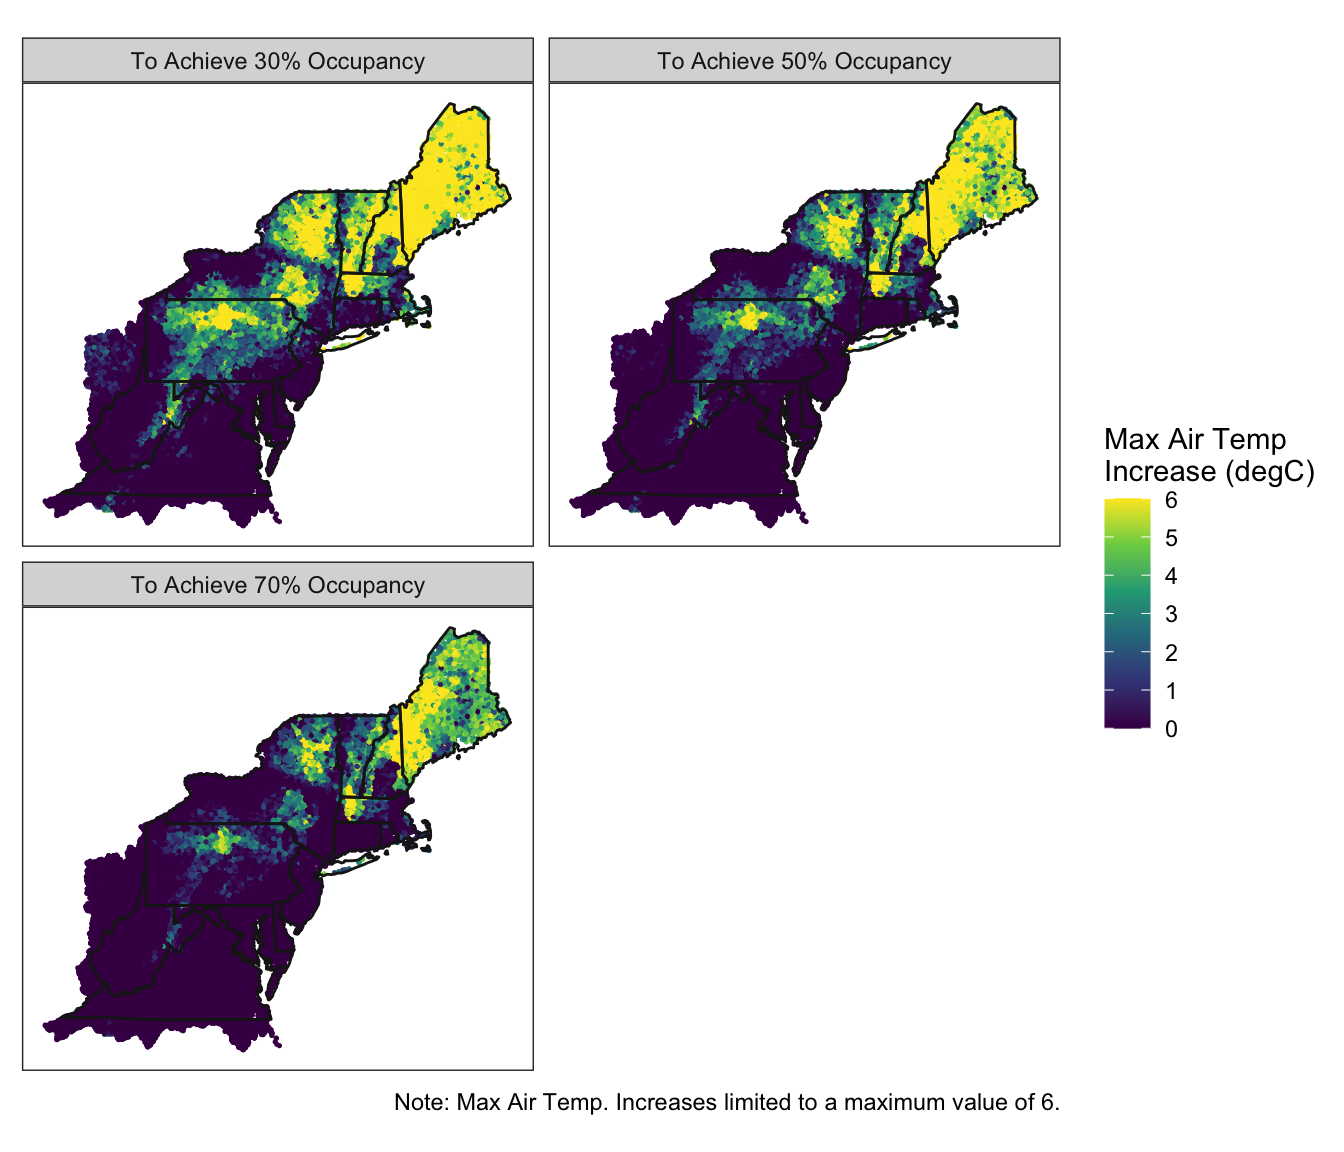
\includegraphics{sheds-bto-model_files/figure-latex/intro-map-max-1.pdf}
\caption{\label{fig:intro-map-max}Predicted Max. Air Temperature Increases to Achieve Varying Occupancy Probabilities}
\end{figure}

The predicted occupancy probabilities along with stream temperature predictions and various catchment characteristics can be found in the \href{https://www.usgs.gov/apps/ecosheds/ice-northeast/}{Northeast Interactive Catchment Explorer (ICE)}. Data files containing the predictions are also available for download (see \protect\hyperlink{downloads}{Downloads}).

The model is periodically updated when either new observation data are available, or following each update of the northeast stream temperature model. Currently, updates are being performed annually, usually in the fall.

\hypertarget{documentation}{%
\section{Documentation}\label{documentation}}

The documentation is divided into the following sections:

\begin{enumerate}
\def\labelenumi{\arabic{enumi}.}
\tightlist
\item
  \protect\hyperlink{intro}{Introduction} provides an overview the model and its documentation
\item
  \protect\hyperlink{data-sources}{Data Sources} describes the data sources and data processing steps used to generate the model inputs and observed data
\item
  \protect\hyperlink{model-development}{Model Development} describes the model structure and implementation
\item
  \protect\hyperlink{calibration-and-validation}{Calibration and Validation} summarizes the model calibration and validation
\item
  \protect\hyperlink{predictions}{Predictions} describes the model prediction scenarios and metrics
\item
  \protect\hyperlink{downloads}{Downloads} provides links to download the model predictions
\item
  \protect\hyperlink{history}{History} contains a list of changes to the model over time
\end{enumerate}

\hypertarget{source-code}{%
\section{Source Code}\label{source-code}}

The source code for the model itself and this documentation is available in the Github repository \href{https://github.com/EcoSHEDS/northeast-bto-model}{walkerjeffd/sheds-bto-model}. Each version of the model will be included under the list of \href{https://github.com/EcoSHEDS/northeast-bto-model/releases}{Releases}.

\hypertarget{data-sources}{%
\chapter{Data Sources}\label{data-sources}}

\hypertarget{catchment-delineation}{%
\section{Catchment Delineation}\label{catchment-delineation}}

The model domain was based on the \href{https://conte-ecology.github.io/shedsGisData/\#the-national-hydrography-dataset-high-resolution-delineation-version-2-nhdhrdv2}{EcoSHEDS Northeast Catchment Delineation}, which is also used for the \href{https://ecosheds.org/models/stream-temperature/latest/}{EcoSHEDS Northeast Stream Temperature Model}. This delineation was created in 2014-2015 to provide a high resolution catchment delineation across the northeast that was spatially consistent over the entire region. The EcoSHEDS delineation was created prior to the completion of the \href{https://www.usgs.gov/national-hydrography/nhdplus-high-resolution}{USGS NHDPlus High Resolution} dataset. Unfortunately, the two delineations are not directly relatable.

Figure \ref{fig:data-catchments} shows the extent of this delineation, which covers the northeast and mid-Atlantic portions of the eastern U.S. from Maine to Virginia. The delineation includes approximately 450,000 individual catchments, with an mean surface area of 1.6 km\textsuperscript{2}.

\begin{figure}
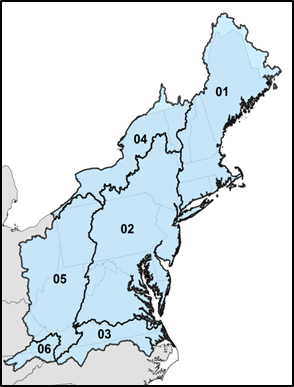
\includegraphics[width=2.94in]{img/hydrologic-regions} \caption{Hydrologic Regions of EcoSHEDS Northeast Catchment Delineation}\label{fig:data-catchments}
\end{figure}

\hypertarget{huc8-basins}{%
\section{HUC8 Basins}\label{huc8-basins}}

The \href{https://water.usgs.gov/GIS/huc.html}{8-digit Hydrologic Unit Code (HUC8)} basins were used to account for regional variations in brook trout occupancy that was not explained by stream temperature data (see {[}Model Structure{]}). Figure \ref{fig:data-huc8} shows the boundary of each HUC8 basin.

\begin{figure}
\centering
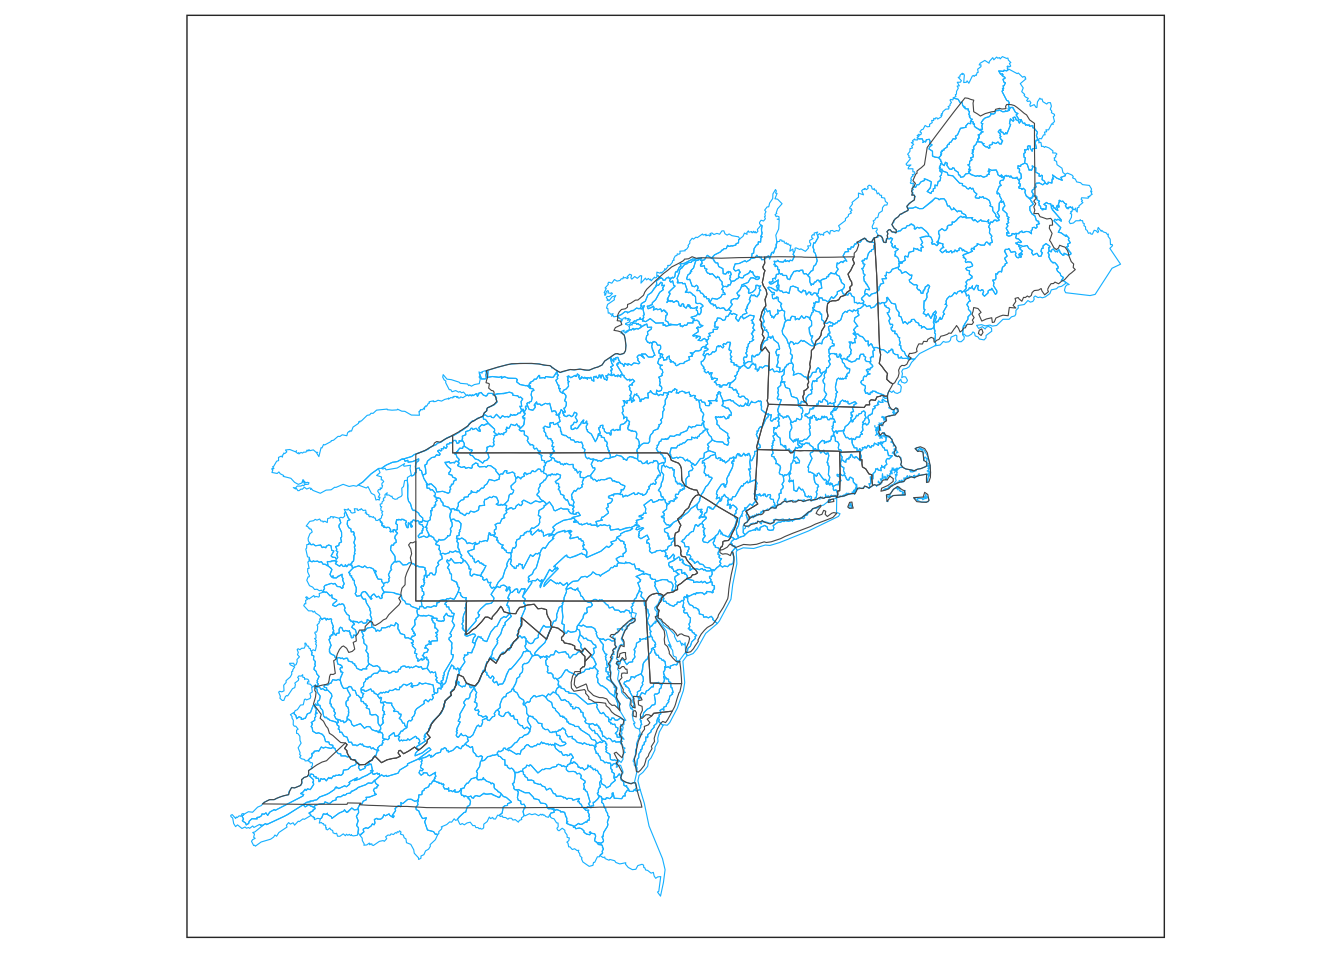
\includegraphics{sheds-bto-model_files/figure-latex/data-huc8-1.pdf}
\caption{\label{fig:data-huc8}HUC8 Basins}
\end{figure}

\hypertarget{observation-data}{%
\section{Observation Data}\label{observation-data}}

Observed presence/absence data of eastern brook trout was gathered from multiple state agencies.

The raw presence/absence observations were aggregated by catchment for input to the model. If there were multiple observations in a single catchment (either at different locations or at different times), then the catchment was assigned to the \texttt{presence} category if there was at least presence among those observations. If all observations were absences, then the catchment was assigned to \texttt{absence}.

The follow map, figures, and table provide a summary of the observed catchment presence/absence by state.

\begin{figure}
\centering
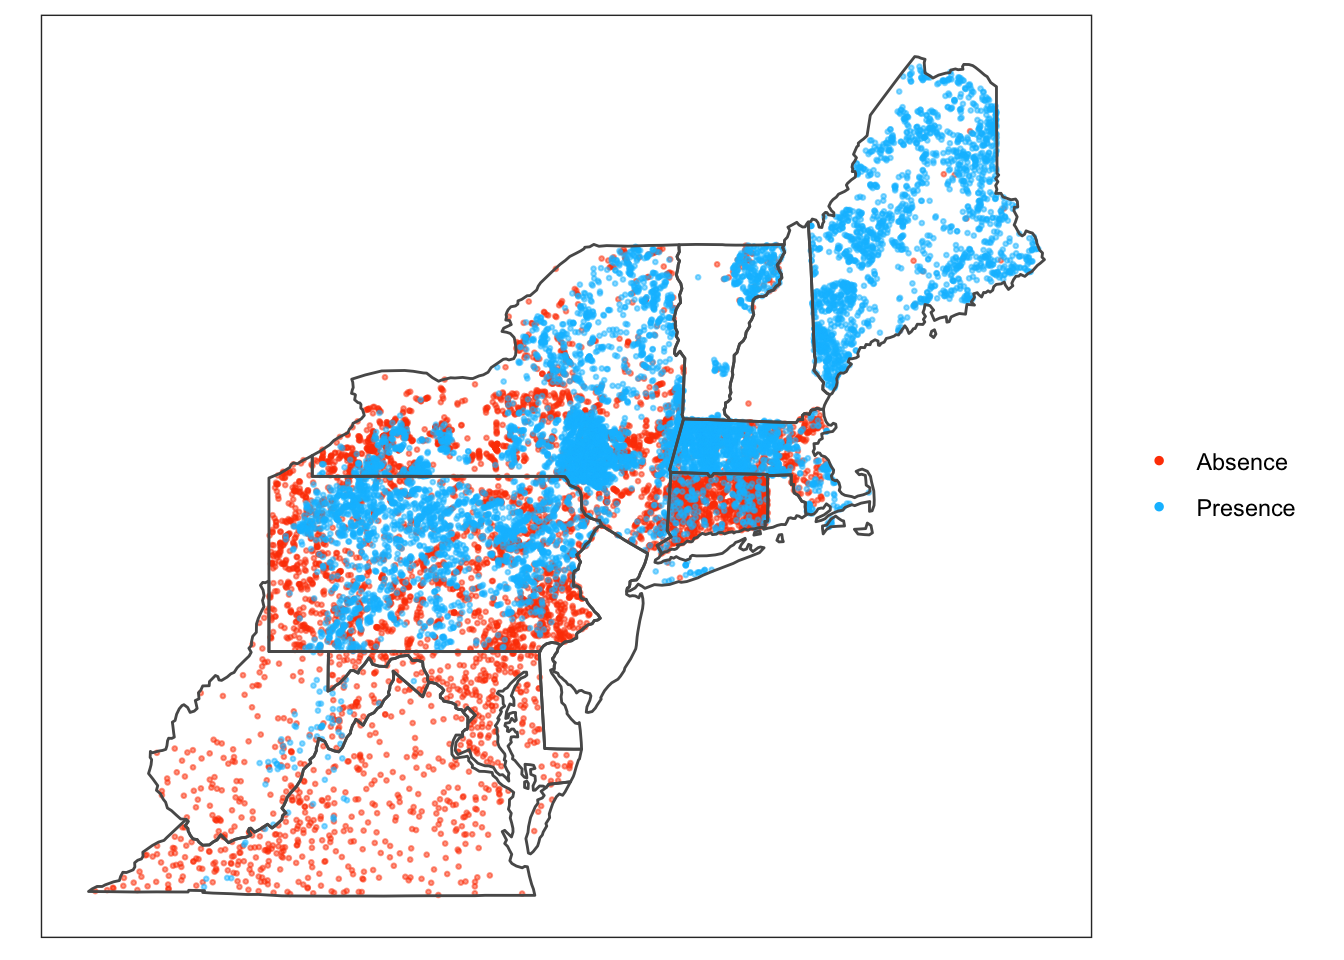
\includegraphics{sheds-bto-model_files/figure-latex/data-obs-map-1.pdf}
\caption{\label{fig:data-obs-map}Map of Presence/Absence by Catchment}
\end{figure}

\begin{figure}
\centering
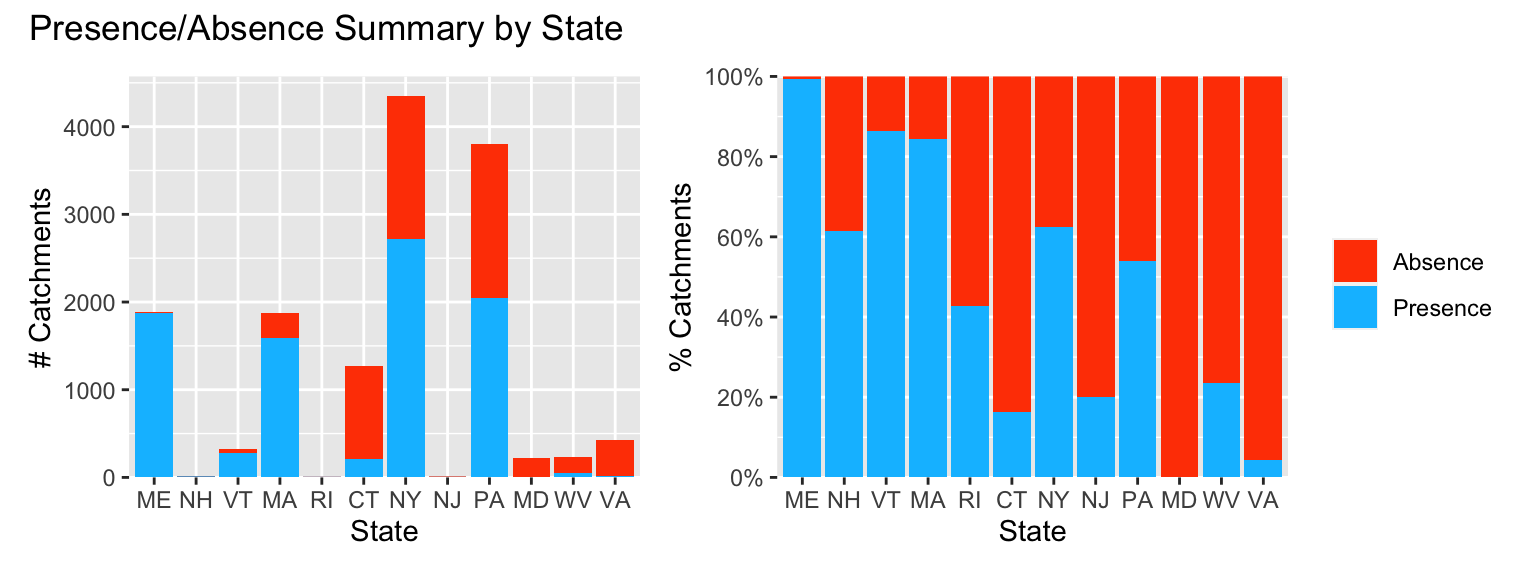
\includegraphics{sheds-bto-model_files/figure-latex/data-obs-state-plot-1.pdf}
\caption{\label{fig:data-obs-state-plot}Presence/Absence Catchment Totals by State}
\end{figure}

\begin{tabular}{l|r|r|r|r}
\hline
State & Presence & Absence & Total & \% Presence\\
\hline
ME & 1,874 & 10 & 1,884 & 99.5\%\\
\hline
NH & 8 & 5 & 13 & 61.5\%\\
\hline
VT & 283 & 45 & 328 & 86.3\%\\
\hline
MA & 1,585 & 294 & 1,879 & 84.4\%\\
\hline
RI & 3 & 4 & 7 & 42.9\%\\
\hline
CT & 206 & 1,066 & 1,272 & 16.2\%\\
\hline
NY & 2,722 & 1,633 & 4,355 & 62.5\%\\
\hline
NJ & 2 & 8 & 10 & 20.0\%\\
\hline
PA & 2,050 & 1,747 & 3,797 & 54.0\%\\
\hline
MD & 0 & 226 & 226 & 0.0\%\\
\hline
WV & 55 & 178 & 233 & 23.6\%\\
\hline
VA & 18 & 404 & 422 & 4.3\%\\
\hline
Total & 8,806 & 5,620 & 14,426 & 61.0\%\\
\hline
\end{tabular}

\hypertarget{stream-temperature}{%
\section{Stream Temperature}\label{stream-temperature}}

The primary input to the brook trout occupancy model is the estimated mean July stream temperature of each catchment. These estimates were generated using the \href{https://ecosheds.org/models/stream-temperature/latest/}{EcoSHEDS Northeast Stream Temperature Model}. The estimated value for each catchment represents the long-term mean July stream temperature computed over all years since 1980. Estimates are only generated for catchments with total cumulative drainage areas less than 200 km\textsuperscript{2} due to the great complexity, anthropogenic impacts, and non-linearities associated with temperature dynamics in larger rivers.

The stream temperature model is based on a linear mixed effects framework that accounts for spatial and temporal correlations using a hierachical Bayesian structure. The primary input variables include air temperature, precipitation, land use (forest, agriculture, high development), impounded drainage area, and total drainage area. See the \href{https://ecosheds.org/models/stream-temperature/latest/}{stream temperature model documentation} for more information.

Figure \ref{fig:data-temp} shows the estimated mean July stream temperature for each catchment.

\begin{figure}
\centering
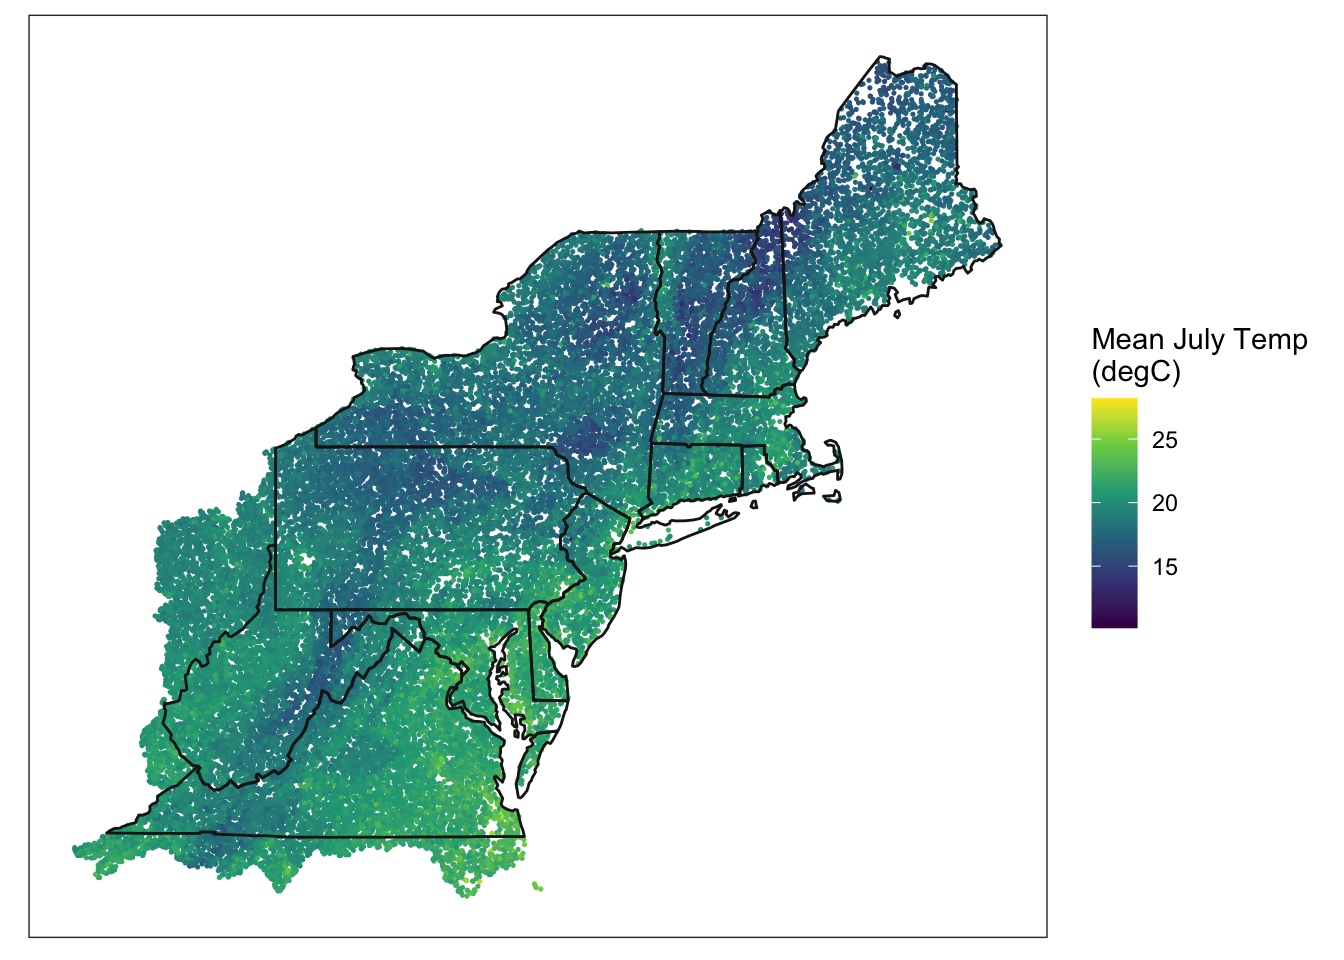
\includegraphics{sheds-bto-model_files/figure-latex/data-temp-1.pdf}
\caption{\label{fig:data-temp}Estimated Mean July Stream Temperature by Catchment}
\end{figure}

\hypertarget{model-development}{%
\chapter{Model Development}\label{model-development}}

\hypertarget{model-definition}{%
\section{Model Definition}\label{model-definition}}

The occupancy model uses a logistic linear mixed effects model framework for estimating the probability of occupancy in each catchment \citep{bolker2009, zuur2009}.

The model includes one fixed effect representing the estimated mean July stream temperature (see \protect\hyperlink{stream-temperature}{Stream Temperature}), and a random effect intercept that varies by HUC8. The random effect is included to account for spatial variations in observed occupancy that are not explained by the mean July stream temperature.

The model is fit using the \texttt{glmer()} function of the \texttt{lme4} R package \citep{bates2015} using the following formula and parameters.

\begin{Shaded}
\begin{Highlighting}[]
\NormalTok{lme4}\SpecialCharTok{::}\FunctionTok{glmer}\NormalTok{(}
\NormalTok{  presence }\SpecialCharTok{\textasciitilde{}}\NormalTok{ mean\_jul\_temp }\SpecialCharTok{+}\NormalTok{ (}\DecValTok{1} \SpecialCharTok{|}\NormalTok{ huc8),}
  \AttributeTok{family =} \FunctionTok{binomial}\NormalTok{(}\AttributeTok{link =} \StringTok{"logit"}\NormalTok{),}
  \AttributeTok{data =}\NormalTok{ model\_data,}
  \AttributeTok{control =} \FunctionTok{glmerControl}\NormalTok{(}\AttributeTok{optimizer =} \StringTok{"bobyqa"}\NormalTok{)}
\NormalTok{)}
\end{Highlighting}
\end{Shaded}

\hypertarget{model-history}{%
\section{Model History}\label{model-history}}

The original development of this model was based on a similar brook trout occupancy model that was developed using a Bayesian hierarchical framework to evaluate associations between various catchment and riparian characteristics as well as climate inputs and the occupancy probability in catchments within the state of Connecticut \citep{kanno2015}.

Prior to version 2.0.0, the EcoSHEDS northeast brook trout occupancy model included a number of independent variables (i.e., covariates) representing land use (forest, agriculture, high intensity development), climate (summer precipitation), and drainage area. The earlier model versions also included the mean July stream temperature as estimated by the EcoSHEDS northeast stream temperature model. However, because the stream temperature model depended on a number of the same independent variables, the estimated effects in the occupancy model were often counter-intuitive due to cross-correlations between some covariates and the estimated stream temperature.

Therefore, beginning with version 2.0.0, the brook trout occupancy model uses only the mean July stream temperature as the sole fixed effect. This change resulted in a small decrease in model accuracy, but provides more intuitive results and can be more easily applied for evaluating alternative climate or land use change scenarios.

\hypertarget{calibration-and-validation}{%
\chapter{Calibration and Validation}\label{calibration-and-validation}}

\hypertarget{dataset-split}{%
\section{Dataset Split}\label{dataset-split}}

To calibrate and validate the model, the observed dataset of presence/absence by catchment (see \protect\hyperlink{observation-data}{Observation Data}) was randomly split using 80\% of the catchments for calibration and 20\% for validation.

\begin{figure}
\centering
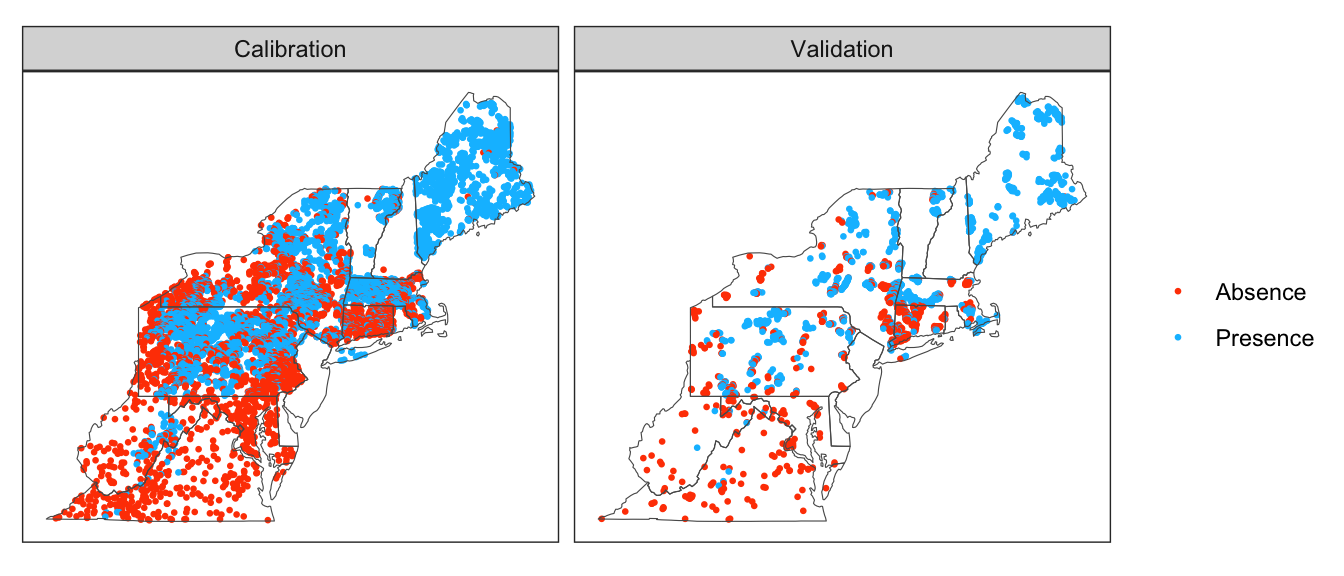
\includegraphics{sheds-bto-model_files/figure-latex/calib-map-1.pdf}
\caption{\label{fig:calib-map}Calibration and Validation Splits}
\end{figure}

\begin{tabular}{l|r|r|r|r}
\hline
Partition & Presence & Absense & Total & \% Presence\\
\hline
Calibration & 6,690 & 3,612 & 10,302 & 64.9\%\\
\hline
Validation & 1,822 & 1,017 & 2,839 & 64.2\%\\
\hline
Total & 8,512 & 4,629 & 13,141 & 64.8\%\\
\hline
\end{tabular}

\hypertarget{calibration}{%
\section{Calibration}\label{calibration}}

The following output summarizes the fitted model using the calibration subset.

\begin{verbatim}
Generalized linear mixed model fit by maximum likelihood (Laplace
  Approximation) [glmerMod]
 Family: binomial  ( logit )
Formula: presence ~ mean_jul_temp + (1 | huc8)
   Data: model_data
Control: glmerControl(optimizer = "bobyqa")

     AIC      BIC   logLik deviance df.resid 
  8592.8   8614.7  -4293.4   8586.8    10934 

Scaled residuals: 
    Min      1Q  Median      3Q     Max 
-32.628  -0.371   0.135   0.427  11.133 

Random effects:
 Groups Name        Variance Std.Dev.
 huc8   (Intercept) 4.999    2.236   
Number of obs: 10937, groups:  huc8, 202

Fixed effects:
              Estimate Std. Error z value Pr(>|z|)    
(Intercept)   19.54035    0.68083   28.70   <2e-16 ***
mean_jul_temp -1.03582    0.03444  -30.07   <2e-16 ***
---
Signif. codes:  0 '***' 0.001 '**' 0.01 '*' 0.05 '.' 0.1 ' ' 1

Correlation of Fixed Effects:
            (Intr)
mean_jl_tmp -0.965
\end{verbatim}

The estimated fixed effect for mean July temp (\texttt{mean\_jul\_temp}) was -1.04. Because the estimated value is negative, the occupancy probability is higher at lower stream temperatures. Figure @\ref(fig:calib-fixed) contains a marginal effects plot showing the predicted probability over varying mean July stream temperatures (excluding random effects).

\begin{figure}
\centering
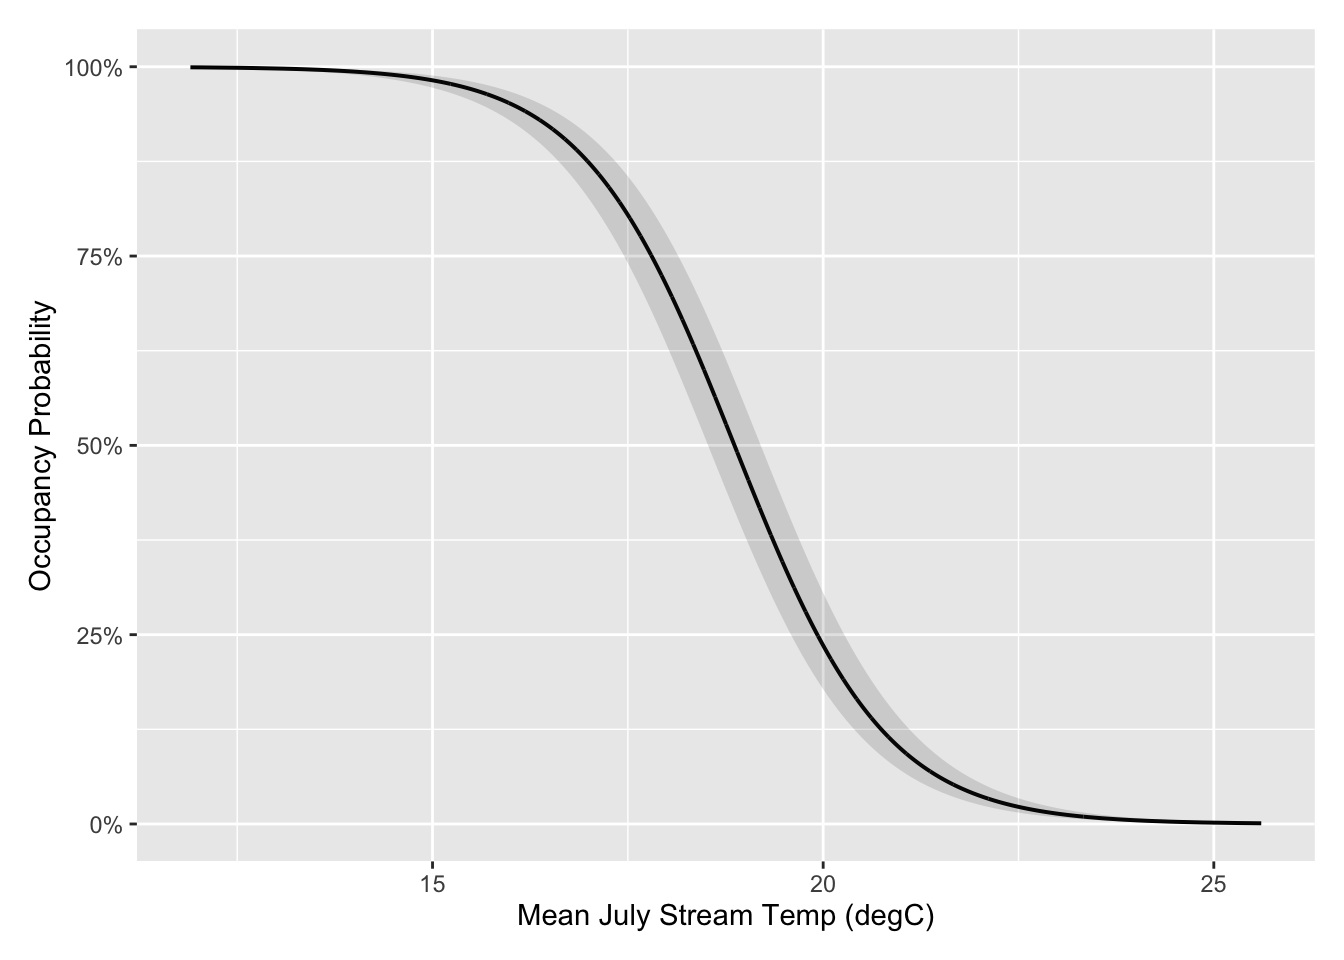
\includegraphics{sheds-bto-model_files/figure-latex/calib-fixef-1.pdf}
\caption{\label{fig:calib-fixef}Marginal Effects Plot for Mean July Stream Temperature.}
\end{figure}

The random effect intercept varies by HUC8 basin. Basins with higher values tend to have higher occupancy probabilities for a given mean July stream temperature. Some HUC8 basins do not have an estimated value because there was no observations with the calibration dataset.

\begin{figure}
\centering
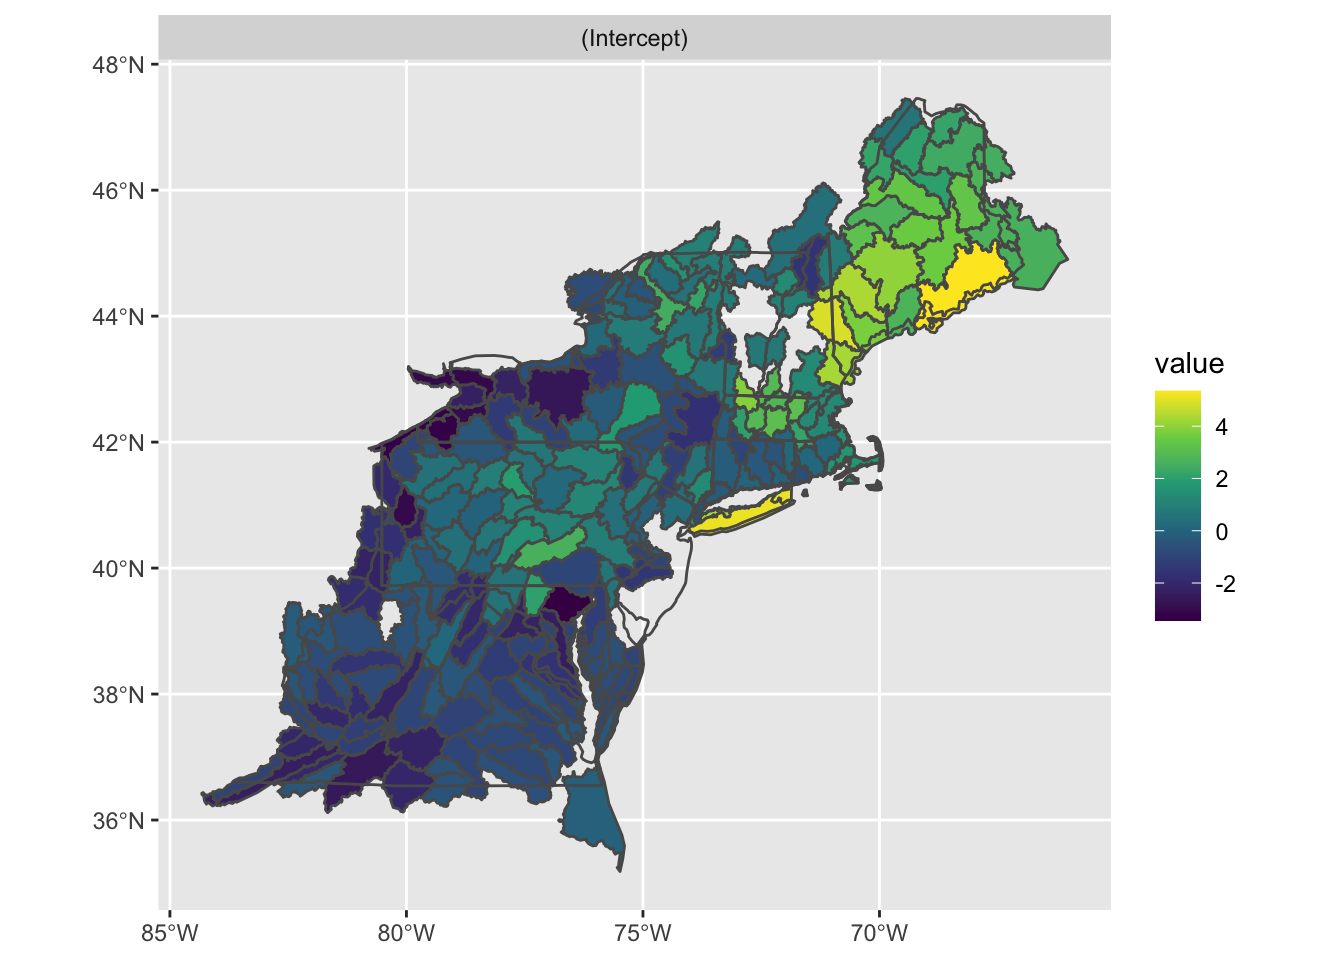
\includegraphics{sheds-bto-model_files/figure-latex/calib-ranef-1.pdf}
\caption{\label{fig:calib-ranef}Random Effect Intercept by HUC8 Basin}
\end{figure}

The model accuracy and performance is summarized by a series of metrics computed from the confusion matrix, which contains the total number of true positives, true negatives, false positives, and false negatives. In the 2x2 table at the top of the following output, the columns (\texttt{Reference}) refer to the observed condition in each catchment (\texttt{1} = presence, \texttt{0} = absence), while the rows (\texttt{Prediction}) refer to the predicted condition. The predicted probabilities were converted to presence/absence using a 50\% cutoff. The remaining output provides a series of performance metrics computed from the confusion matrix using the \texttt{confusionMatrix()} of the \texttt{caret} package \citep{kuhn2022}. See the \href{https://rdrr.io/cran/caret/man/confusionMatrix.html}{help page} for that function, as well as \href{https://en.wikipedia.org/wiki/Confusion_matrix}{this Wikipedia article}, for definitions of each metric.

\begin{verbatim}
Confusion Matrix and Statistics

          Reference
Prediction    0    1
         0 2733  728
         1 1107 6369
                                          
               Accuracy : 0.8322          
                 95% CI : (0.8251, 0.8392)
    No Information Rate : 0.6489          
    P-Value [Acc > NIR] : < 2.2e-16       
                                          
                  Kappa : 0.6233          
                                          
 Mcnemar's Test P-Value : < 2.2e-16       
                                          
            Sensitivity : 0.8974          
            Specificity : 0.7117          
         Pos Pred Value : 0.8519          
         Neg Pred Value : 0.7897          
             Prevalence : 0.6489          
         Detection Rate : 0.5823          
   Detection Prevalence : 0.6836          
      Balanced Accuracy : 0.8046          
                                          
       'Positive' Class : 1               
                                          
\end{verbatim}

\hypertarget{validation}{%
\section{Validation}\label{validation}}

Using the calibrated model, predicted probabilities were computed using the indendent validation dataset.

The confusion matrix for the validation dataset indicates slightly lower accuracy (0.83 vs 0.81), but overall comparable performance. These results suggest that the model does not suffer from overfitting.

\begin{verbatim}
Confusion Matrix and Statistics

          Reference
Prediction    0    1
         0  590  221
         1  199 1194
                                          
               Accuracy : 0.8094          
                 95% CI : (0.7924, 0.8256)
    No Information Rate : 0.642           
    P-Value [Acc > NIR] : <2e-16          
                                          
                  Kappa : 0.588           
                                          
 Mcnemar's Test P-Value : 0.3055          
                                          
            Sensitivity : 0.8438          
            Specificity : 0.7478          
         Pos Pred Value : 0.8571          
         Neg Pred Value : 0.7275          
             Prevalence : 0.6420          
         Detection Rate : 0.5417          
   Detection Prevalence : 0.6320          
      Balanced Accuracy : 0.7958          
                                          
       'Positive' Class : 1               
                                          
\end{verbatim}

The following table compares the performance metrics between the two subsets.

\begin{tabular}{l|r|r}
\hline
Metric & Calibration & Validation\\
\hline
Accuracy & 0.832 & 0.809\\
\hline
Sensitivity & 0.897 & 0.844\\
\hline
Specificity & 0.712 & 0.748\\
\hline
Pos Pred Value & 0.852 & 0.857\\
\hline
Neg Pred Value & 0.790 & 0.727\\
\hline
Precision & 0.852 & 0.857\\
\hline
Recall & 0.897 & 0.844\\
\hline
F1 & 0.874 & 0.850\\
\hline
Prevalence & 0.649 & 0.642\\
\hline
Detection Rate & 0.582 & 0.542\\
\hline
Detection Prevalence & 0.684 & 0.632\\
\hline
Balanced Accuracy & 0.805 & 0.796\\
\hline
\end{tabular}

Lastly, \href{https://en.wikipedia.org/wiki/Receiver_operating_characteristic}{Receiver Operator Characteristic (ROC)} curves and Area Under the Curve (AUC) values also shows comparable performance between the calibration and validation subsets.

\begin{figure}
\centering
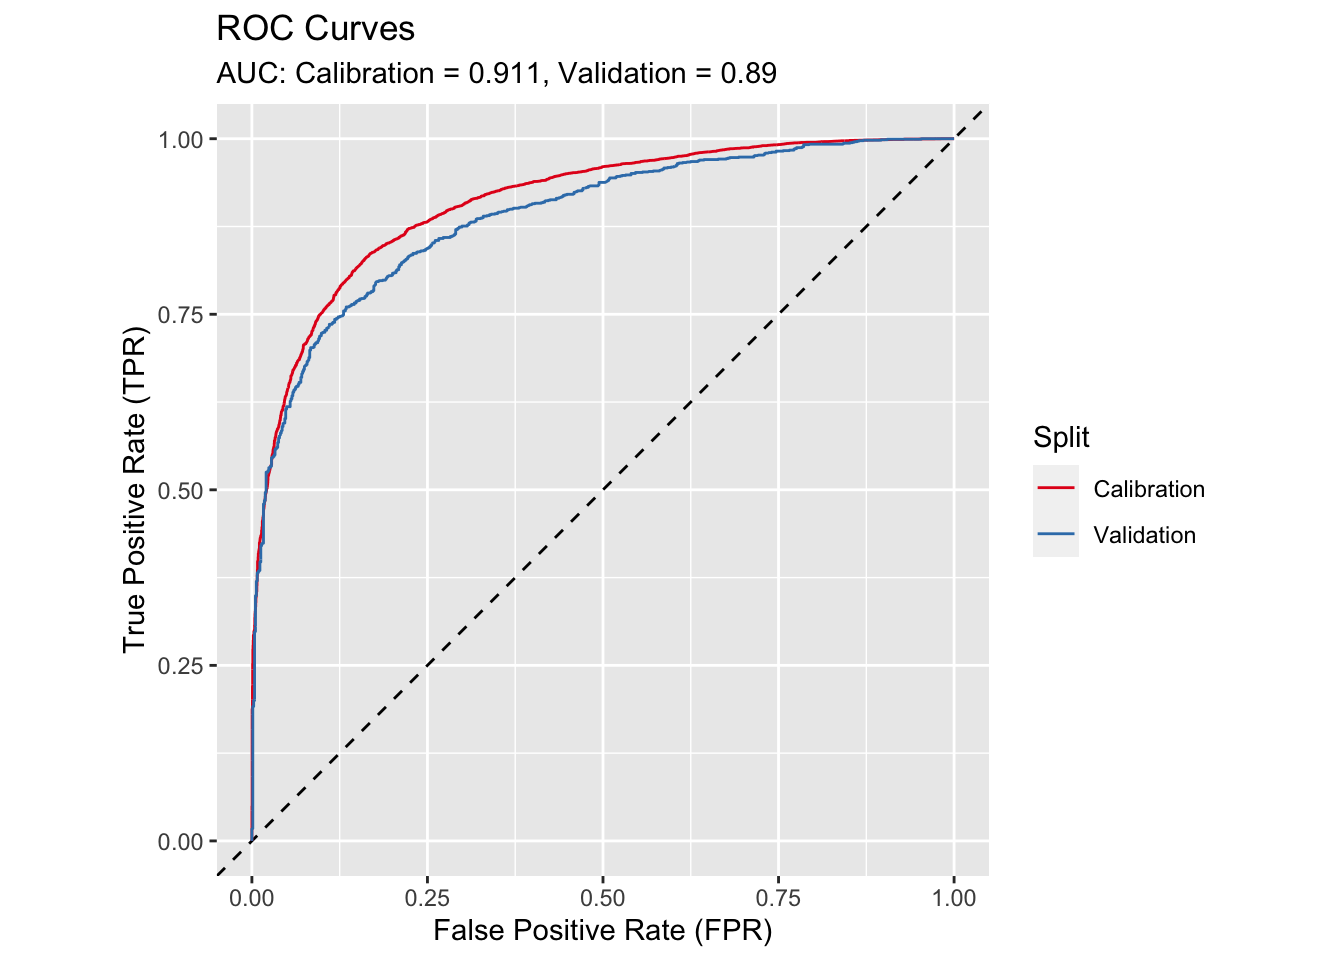
\includegraphics{sheds-bto-model_files/figure-latex/calib-roc-1.pdf}
\caption{\label{fig:calib-roc}ROC Curves for Calibration and Validation}
\end{figure}

\hypertarget{predictions}{%
\chapter{Predictions}\label{predictions}}

\hypertarget{full-calibration}{%
\section{Full Calibration}\label{full-calibration}}

To utilize the maximum amount of information available from the observation data, the model was re-calibrated using the full observation dataset. The following output shows that the estimated effects were comparable to those from the initial calibration based on 80\% split of the full dataset (see \protect\hyperlink{calibration}{Calibration}).

\begin{verbatim}
Generalized linear mixed model fit by maximum likelihood (Laplace
  Approximation) [glmerMod]
 Family: binomial  ( logit )
Formula: presence ~ mean_jul_temp + (1 | huc8)
   Data: predict_inp
Control: glmerControl(optimizer = "bobyqa")

     AIC      BIC   logLik deviance df.resid 
 10286.4  10308.9  -5140.2  10280.4    13138 

Scaled residuals: 
     Min       1Q   Median       3Q      Max 
-29.1602  -0.3739   0.1199   0.4331  10.7152 

Random effects:
 Groups Name        Variance Std.Dev.
 huc8   (Intercept) 5.148    2.269   
Number of obs: 13141, groups:  huc8, 209

Fixed effects:
              Estimate Std. Error z value Pr(>|z|)    
(Intercept)   18.43567    0.61595   29.93   <2e-16 ***
mean_jul_temp -0.97728    0.03084  -31.69   <2e-16 ***
---
Signif. codes:  0 '***' 0.001 '**' 0.01 '*' 0.05 '.' 0.1 ' ' 1

Correlation of Fixed Effects:
            (Intr)
mean_jl_tmp -0.958
\end{verbatim}

The estimated fixed effect for mean July temp (\texttt{mean\_jul\_temp}) was -0.98. Figure @ref(fig:Calibration and Validation) contains a marginal effects plot showing the predicted probability over varying mean July stream temperatures (excluding random effects) showing higher predicted probabilities at lower stream temperatures.

\begin{figure}
\centering
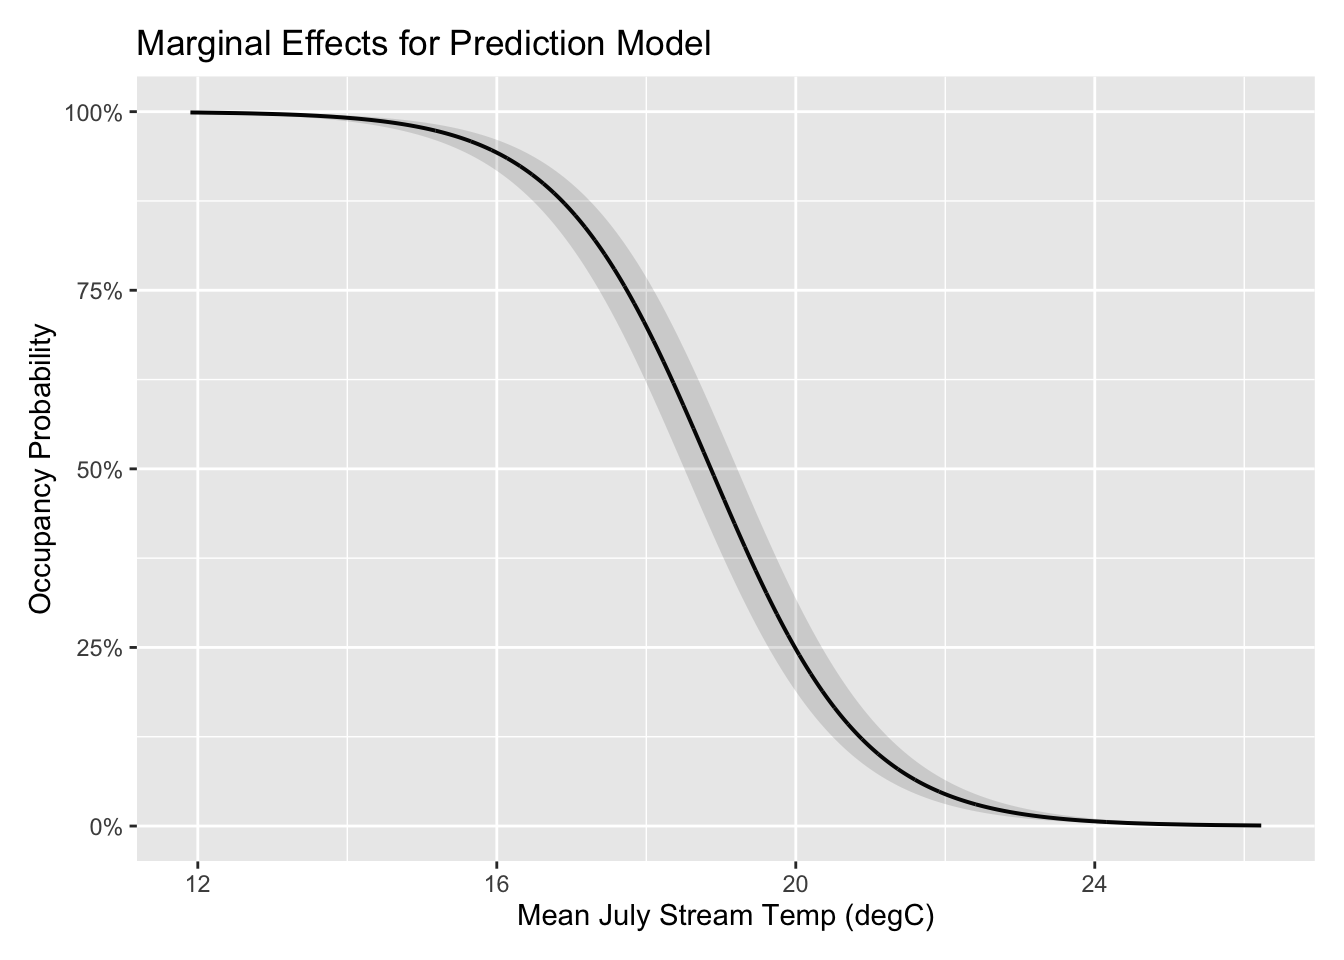
\includegraphics{sheds-bto-model_files/figure-latex/predict-model-fixef-1.pdf}
\caption{\label{fig:predict-model-fixef}Marginal Effects Plot for Mean July Stream Temperature (Prediction Model)}
\end{figure}

The HUC8 random effect intercepts were also relatively similar to those from the initial calibration model.

\begin{figure}
\centering
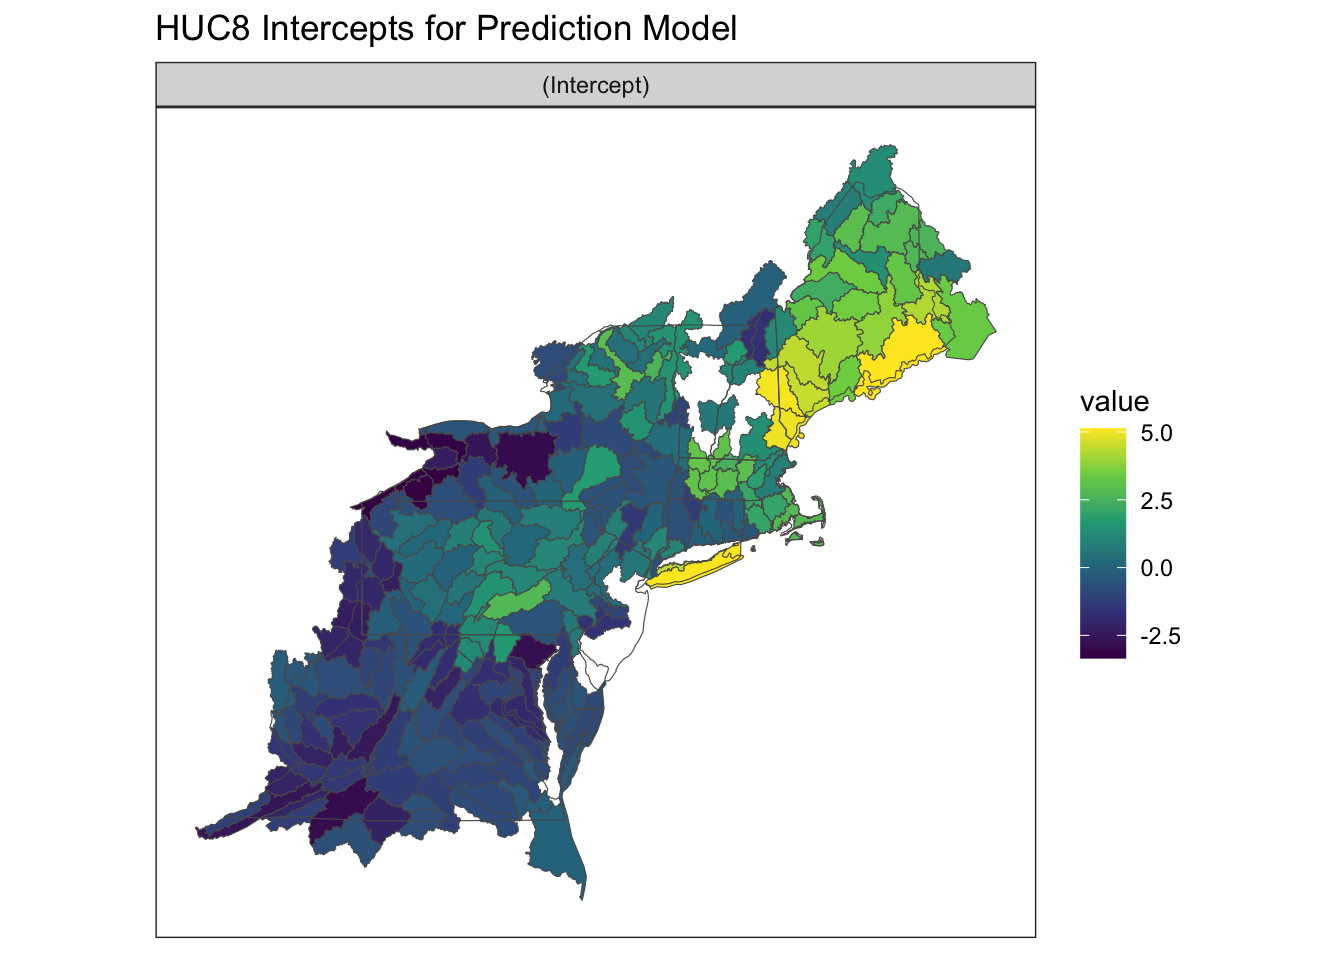
\includegraphics{sheds-bto-model_files/figure-latex/predict-model-ranef-1.pdf}
\caption{\label{fig:predict-model-ranef}Random Effect Intercept by HUC8 Basin (Prediction Model)}
\end{figure}

The following output summarizes the prediction model's accuracy and performance (see \protect\hyperlink{calibration}{Calibration} for explanation of this output).

\begin{verbatim}
Confusion Matrix and Statistics

          Reference
Prediction    0    1
         0 3319  902
         1 1310 7610
                                         
               Accuracy : 0.8317         
                 95% CI : (0.8252, 0.838)
    No Information Rate : 0.6477         
    P-Value [Acc > NIR] : < 2.2e-16      
                                         
                  Kappa : 0.6236         
                                         
 Mcnemar's Test P-Value : < 2.2e-16      
                                         
            Sensitivity : 0.8940         
            Specificity : 0.7170         
         Pos Pred Value : 0.8531         
         Neg Pred Value : 0.7863         
             Prevalence : 0.6477         
         Detection Rate : 0.5791         
   Detection Prevalence : 0.6788         
      Balanced Accuracy : 0.8055         
                                         
       'Positive' Class : 1              
                                         
\end{verbatim}

The following table compares the performance of the prediction model using all available data to that of the calibration and validation subsets (see \protect\hyperlink{calibration-and-validation}{Calibration and Validation}). Overall, the full prediction model performs very similarly to the initial calibration model.

\begin{tabular}{l|r|r|r}
\hline
Metric & Calibration & Validation & Full (Prediction)\\
\hline
Accuracy & 0.832 & 0.809 & 0.832\\
\hline
Sensitivity & 0.897 & 0.844 & 0.894\\
\hline
Specificity & 0.712 & 0.748 & 0.717\\
\hline
Pos Pred Value & 0.852 & 0.857 & 0.853\\
\hline
Neg Pred Value & 0.790 & 0.727 & 0.786\\
\hline
Precision & 0.852 & 0.857 & 0.853\\
\hline
Recall & 0.897 & 0.844 & 0.894\\
\hline
F1 & 0.874 & 0.850 & 0.873\\
\hline
Prevalence & 0.649 & 0.642 & 0.648\\
\hline
Detection Rate & 0.582 & 0.542 & 0.579\\
\hline
Detection Prevalence & 0.684 & 0.632 & 0.679\\
\hline
Balanced Accuracy & 0.805 & 0.796 & 0.806\\
\hline
\end{tabular}

\hypertarget{prediction-metrics}{%
\section{Prediction Metrics}\label{prediction-metrics}}

Using the prediction model that was fitted to the full observation dataset, a series of occupancy metrics were computed for each catchment over the region (excluding those with cumulative drainage areas \textgreater{} 200 km\textsuperscript{2}).

The prediction metrics include:

\begin{enumerate}
\def\labelenumi{\arabic{enumi}.}
\tightlist
\item
  Occupancy probability under historical conditions as well as air temperature increases of +2, +4, and +6 degC, which represents a series of simple climate change scenarios.
\end{enumerate}

\begin{figure}
\centering
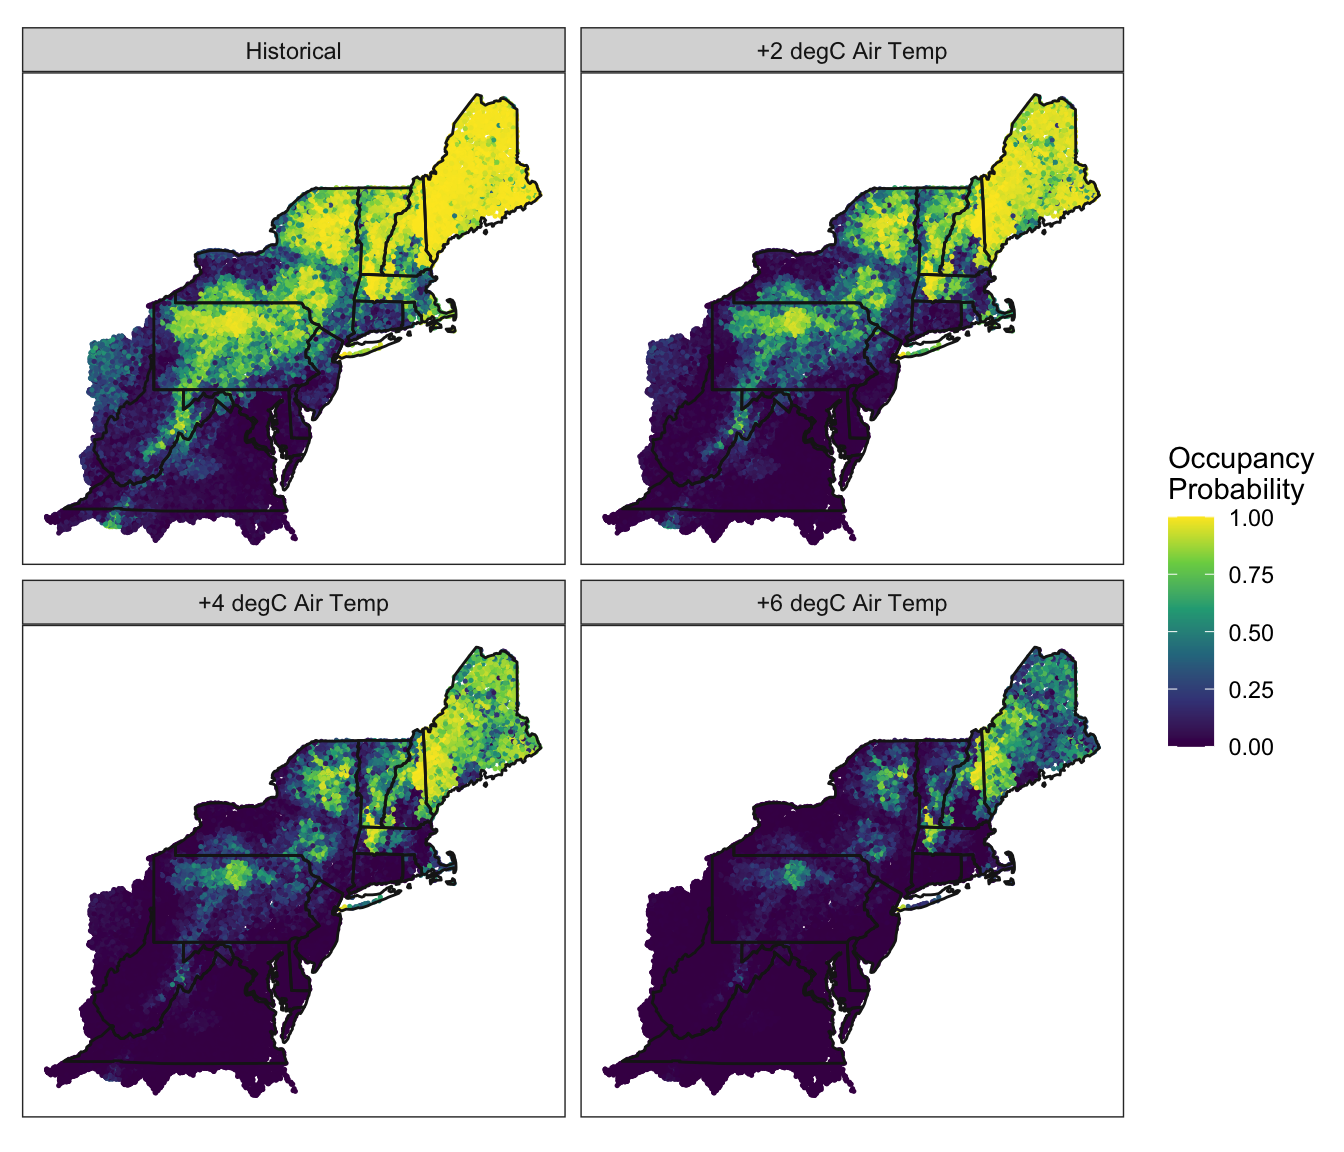
\includegraphics{sheds-bto-model_files/figure-latex/predict-map-prob-1.pdf}
\caption{\label{fig:predict-map-prob}Predicted Occupancy Probabilities under Historical and Future Climate Change Scenarios}
\end{figure}

\begin{enumerate}
\def\labelenumi{\arabic{enumi}.}
\setcounter{enumi}{1}
\tightlist
\item
  The maximum increase in air temperature such that the predicted occupancy would be 30, 50, or 70\%. These metrics indicate how resistant each catchment is to future climate change. Catchments with higher values can tolerate a larger increase in air temperature and still achieve each target occupancy probability.
\end{enumerate}

\begin{figure}
\centering
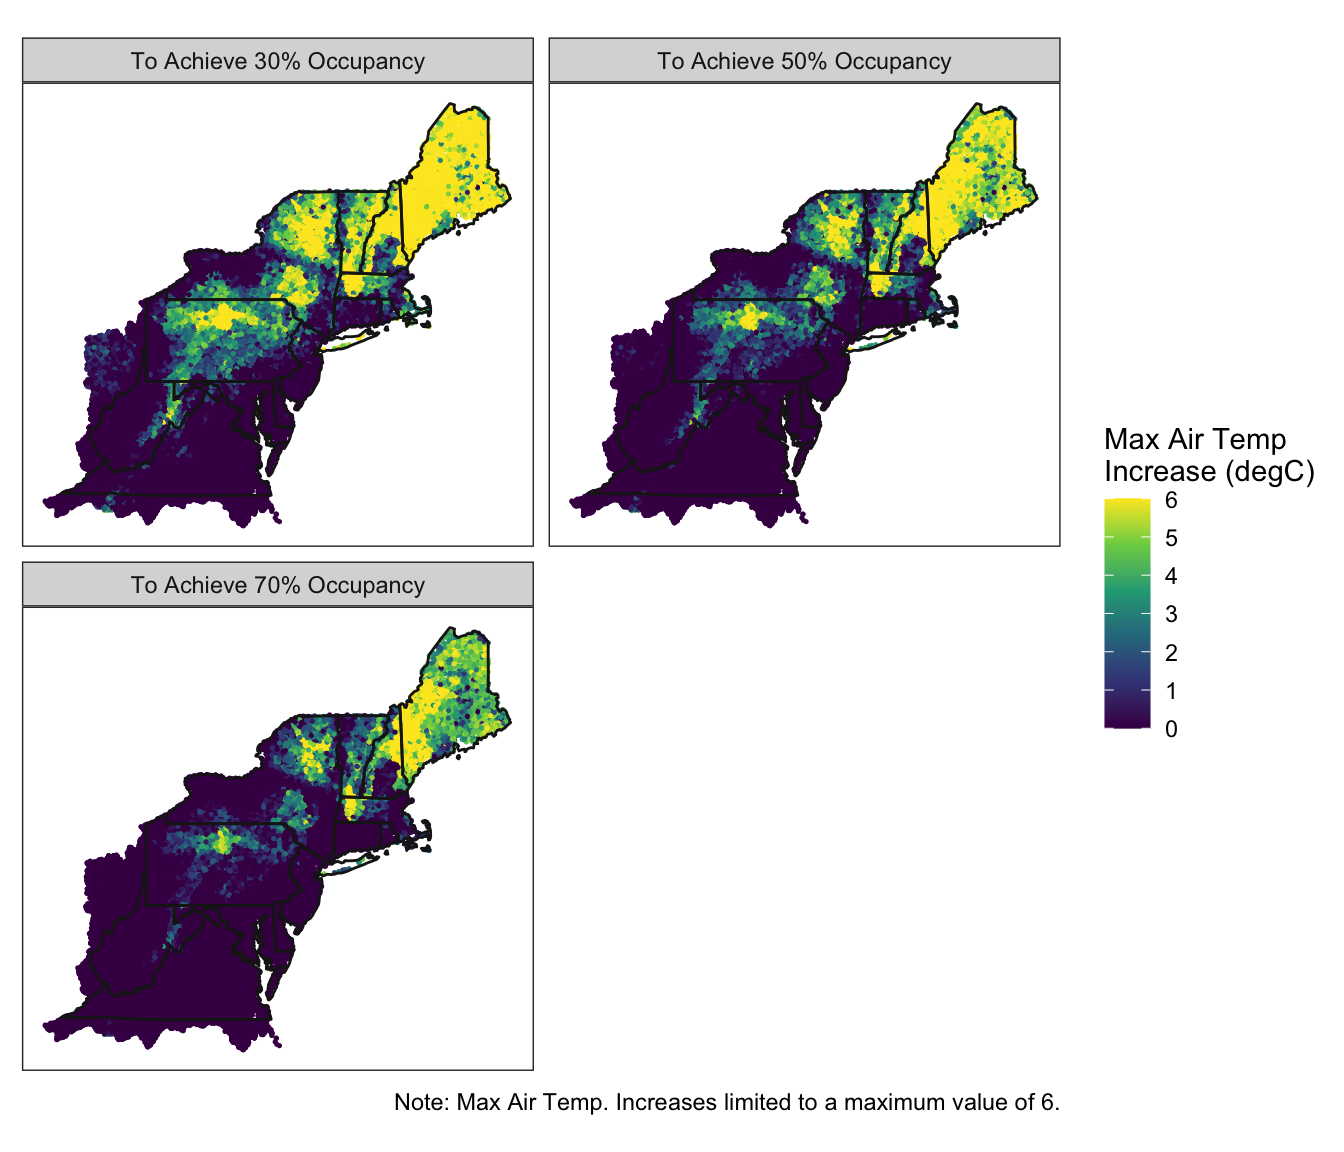
\includegraphics{sheds-bto-model_files/figure-latex/predict-map-max-1.pdf}
\caption{\label{fig:predict-map-max}Predicted Max. Air Temperature Increases to Achieve Varying Occupancy Probabilities}
\end{figure}

A dataset containing the predicted values for these metrics can be downloaded in the \protect\hyperlink{downloads}{Downloads} section.

\hypertarget{downloads}{%
\chapter{Downloads}\label{downloads}}

\hypertarget{model-predictions}{%
\section{Model Predictions}\label{model-predictions}}

The EcoSHEDS Northeast Brook Trout Occupancy Model predictions can be downloaded as CSV file from the following link.

\begin{quote}
\textbf{\href{output/ecosheds-bto-model-v2.0.0.csv}{Brook Trout Occupancy Predictions 2.0.0 (csv)}}
\end{quote}

This file contains the following headers:

\begin{tabular}{r|l}
\hline
CSV Column & Description\\
\hline
featureid & Catchment ID\\
\hline
huc8 & HUC8 ID\\
\hline
mean\_jul\_temp & Mean July Stream Temp. (degC)\\
\hline
occ\_current & Occupancy Probability (Historical)\\
\hline
occ\_air\_2 & Occupancy Probability (+2.0 degC Air Temp)\\
\hline
occ\_air\_4 & Occupancy Probability (+4.0 degC Air Temp)\\
\hline
occ\_air\_6 & Occupancy Probability (+6.0 degC Air Temp)\\
\hline
max\_air\_occ30 & Max Air Temp Increase (degC) for 30\% Occupancy Probability\\
\hline
max\_air\_occ50 & Max Air Temp Increase (degC) for 50\% Occupancy Probability\\
\hline
max\_air\_occ70 & Max Air Temp Increase (degC) for 70\% Occupancy Probability\\
\hline
\end{tabular}

\hypertarget{catchment-delineation-1}{%
\section{Catchment Delineation}\label{catchment-delineation-1}}

The \href{http://conte-ecology.github.io/shedsGisData/}{EcoSHEDS Northeast Catchment Delineation} can be downloaded from the following links, which contain shapefiles grouped by HUC2 region. The model predictions dataset can be joined to these shapefiles using the common \texttt{featureid} column, which serves as the unique catchment ID.

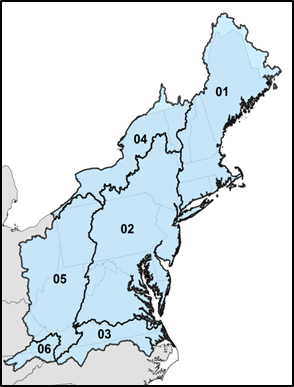
\includegraphics[width=4.08in]{img/hydrologic-regions}

\begin{itemize}
\tightlist
\item
  \href{http://ecosheds.org/assets/nhdhrd/v2/spatial_01.zip}{Region 01 Catchments (zip)}
\item
  \href{http://ecosheds.org/assets/nhdhrd/v2/spatial_02.zip}{Region 02 Catchments (zip)}
\item
  \href{http://ecosheds.org/assets/nhdhrd/v2/spatial_03.zip}{Region 03 Catchments (zip)}
\item
  \href{http://ecosheds.org/assets/nhdhrd/v2/spatial_04.zip}{Region 04 Catchments (zip)}
\item
  \href{http://ecosheds.org/assets/nhdhrd/v2/spatial_05.zip}{Region 05 Catchments (zip)}
\item
  \href{http://ecosheds.org/assets/nhdhrd/v2/spatial_06.zip}{Region 06 Catchments (zip)}
\end{itemize}

The documentation for the catchment delineation is also available:

\begin{quote}
\textbf{\href{http://ecosheds.org/assets/nhdhrd/v2/NHDHRDV2_Documentation.docx}{EcoSHEDS Northeast Catchment Delineation (docx)}}
\end{quote}

\hypertarget{history}{%
\chapter{History}\label{history}}

\hypertarget{versioning}{%
\section{Versioning}\label{versioning}}

The model uses semantic versioning of the form: \texttt{vX.Y.Z}

\begin{itemize}
\tightlist
\item
  \texttt{X} is the \textbf{major} version, which will be incremented when there is a new set of results and major changes to the model structure, code, or datasets.
\item
  \texttt{Y} is the \textbf{minor} version, which will be incremented when there is a new set of results and minor changes in the model code or datasets (but no change in model structure).
\item
  \texttt{Z} is the \textbf{patch} version, which will be incremented only when there is a change to the documentation or code that \emph{does not} yield different results.
\end{itemize}

\hypertarget{change-log}{%
\section{Change Log}\label{change-log}}

\begin{itemize}
\tightlist
\item
  v2.0.0 \textbar{} Jul 8, 2022
  Removed all fixed effects except for mean July stream temperature due to cross-correlation between stream temperatures and other covariates (e.g., forest cover). Changed random effect levels from HUC10 to HUC8.
\item
  v1.4.0 \textbar{} Sep 8, 2021\\
  Re-calibrate model with updated stream temperature model results through 2020 (\href{http://ecosheds.org/models/stream-temperature/v1.3.0/}{v1.3.0}), removed July stream temperature scenarios from predictions (these have been replaced by the air temperature scenarios)
\item
  v1.3.0 \textbar{} Jul 13, 2020\\
  Re-run calibration with updated stream temperature model results through 2019 (\href{http://ecosheds.org/models/stream-temperature/v1.2.0/}{v1.2.0})
\item
  v1.2.2 \textbar{} Jan 17, 2020\\
  Rename prediction metrics to be more consistent
\item
  v1.2.1 \textbar{} Jan 16, 2020\\
  Added predictions for air temperature scenarios (+2, +4, +6 degC), remove 0.5 degC increments from July stream temperature scenarios, revise method for estimating max temperature increases to achieve occupancy thresholds using linear interpolation
\item
  v1.2.0 \textbar{} Dec 3, 2019\\
  Re-run calibration with updated stream temperature model results (\href{http://ecosheds.org/models/stream-temperature/v1.1/}{v1.1})
\item
  v1.1.1 \textbar{} Mar 26, 2019\\
  Update documentation, add {[}Download{]} section containing links to model predictions, catchment delineation, and covariates.
\item
  v1.1.0 \textbar{} Mar 25, 2019\\
  Add observation data from MA DFW. Recalibrate model using \href{http://ecosheds.org/models/stream-temperature/v1.0.1/}{v1.0 of stream temperature model}.
\item
  v1.0.0 \textbar{} Oct 25, 2018\\
  Recalibrate model using \href{http://ecosheds.org/models/stream-temperature/v1.0.1/}{v1.0 of stream temperature model}.
\item
  v0.9.0 \textbar{} Aug 16, 2018\\
  Preliminary release of the new model framework and documentation.
\item
  \textbf{\href{http://conte-ecology.github.io/Northeast_Bkt_Occupancy/}{Previous Versions} (prior to 2018)}\\
  Previous versions of the brook trout occupancy model can be found \href{http://conte-ecology.github.io/Northeast_Bkt_Occupancy/}{here}. That website is now deprecated, but will remain available for future reference. Beginning with v1.0.0 of the new framework and codebase, all model changes and results will be tracked and made available.
\end{itemize}

  \bibliography{references.bib}

\end{document}
